\section{Results}

\subsection{Evaluation of clustering methods}

TODO start with setup and show all parameters to be used 

TODO go through the whole process and show best accuracies in the end



The goal of this evaluation is to find an accurat clustering method for working with news articles. The most suitable algorithm will then be used for the online approach of detecting changes in a news stream based on stories.

\begin{table}[h]
    \centering
    \scalebox{0.6}{
    \begin{tabular}{|l|rrrrr|rrrrr|}
        \hline
        \textbf{HDBSCAN} & \multicolumn{5}{ |c| }{\textbf{Bag of Words}} & \multicolumn{5}{ |c| }{\textbf{Tfidf}} \\
        \hline
        Parameter & Full Text &  Keyterms & Entities & Lemmatized & Stemmed & Full Text &  Keyterms & Entities & Lemmatized & Stemmed \\
        \hline
        min\_size: 2, metric: cosine    & 0.289 & 0.265 & 0.223 & \textbf{0.305} & 0.297 & 0.286     & 0.268 & 0.26      & 0.296     & 0.3       \\
        min\_size: 2, metric: euclidean & 0.101 & 0.093 & 0.110 & 0.101     & 0.106 & 0.301     & 0.170 & 0.241     & \textbf{0.306} & 0.301     \\
        min\_size: 3, metric: cosine    & 0.488 & 0.456 & 0.465 & 0.48      & 0.487 & 0.472     & 0.446 & 0.457     & \textbf{0.493} & 0.478     \\
        min\_size: 3, metric: euclidean & 0.172 & 0.129 & 0.176 & 0.174     & 0.182 & 0.472     & 0.306 & 0.464     & \textbf{0.500} & 0.478     \\
        min\_size: 4, metric: cosine    & 0.630 & 0.555 & 0.625 & 0.552     & 0.577 & 0.577     & 0.586 & \textbf{0.646} & 0.589     & 0.581     \\
        min\_size: 4, metric: euclidean & 0.320 & 0.182 & 0.214 & 0.315     & 0.332 & 0.611     & 0.416 & 0.559     & 0.613     & \textbf{0.615} \\
        min\_size: 5, metric: cosine    & 0.716 & 0.652 & 0.656 & \textbf{0.718} & 0.718 & 0.688     & 0.664 & 0.632     & 0.686     & 0.692     \\
        min\_size: 5, metric: euclidean & 0.355 & 0.217 & 0.266 & 0.41      & 0.389 & \textbf{0.703} & 0.512 & 0.607     & 0.686     & 0.692     \\
        min\_size: 6, metric: cosine    & 0.693 & 0.715 & 0.608 & 0.701     & 0.708 & 0.738     & 0.729 & 0.613     & \textbf{0.751} & 0.747     \\
        min\_size: 6, metric: euclidean & 0.179 & 0.280 & 0.292 & 0.202     & 0.164 & 0.738     & 0.408 & 0.622     & \textbf{0.778} & 0.763     \\
        min\_size: 7, metric: cosine    & 0.631 & 0.611 & 0.552 & 0.643     & 0.634 & 0.689     & 0.685 & 0.553     & 0.718     & \textbf{0.722} \\
        min\_size: 7, metric: euclidean & 0.122 & 0.392 & 0.307 & 0.073     & 0.099 & 0.689     & 0.336 & 0.539     & 0.718     & \textbf{0.722} \\
        min\_size: 8, metric: cosine    & 0.571 & 0.603 & 0.514 & 0.592     & 0.574 & 0.685     & 0.647 & 0.531     & \textbf{0.711} & 0.695     \\
        min\_size: 8, metric: euclidean & 0.056 & 0.339 & 0.338 & 0.025     & 0.057 & 0.685     & 0.286 & 0.522     & \textbf{0.711} & 0.695     \\
        min\_size: 9, metric: cosine    & 0.542 & 0.569 & 0.476 & 0.544     & 0.541 & 0.602     & 0.614 & 0.499     & 0.637     & \textbf{0.640} \\
        min\_size: 9, metric: euclidean & 0.065 & 0.236 & 0.310 & 0.025     & 0.033 & 0.602     & 0.216 & 0.475     & 0.637     & \textbf{0.640} \\
        \hline
        n\_cluster: n\_true              & 0.531 & 0.588 & 0.514 & 0.536     & 0.536 & \textbf{0.713} & 0.653 & 0.584     & 0.672     & 0.693     \\
        \hline
    
    \end{tabular}   
    }
    \caption{Accuracy for each combination of parameter and preprocessing}
    \label{tab:cluster_parameters}
\end{table}   

To begin the evaluation, we first compare six different clustering methods with each other. K-means is included as a baseline, to put the scores in relation to one of the most commonly used clustering algorithms. As we can see in figure \ref{fig:different_clusterings}, HDBSCAN provides the highest accuracy, while being still being one of the fastest algorithms. Based on this data, we can assume HDBSCAN to be a good candidate to work with further. Therefore we focus on this algorithm for the rest of the evaluation to get more insight into its performance and other important properties.

\begin{figure}[h]
    \centering
    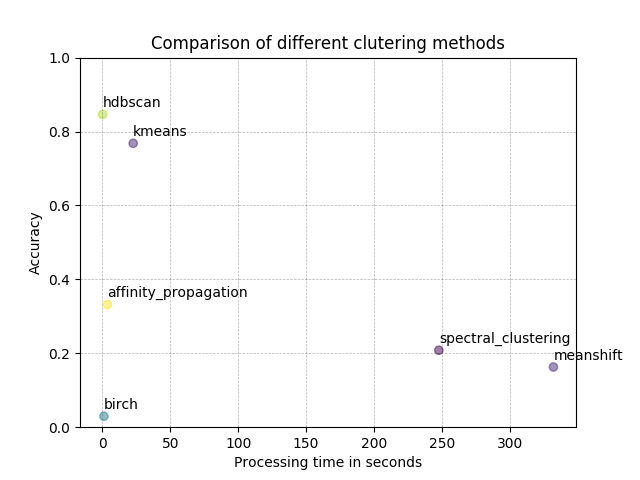
\includegraphics[width=0.5\textwidth]{different_clusterings}
    \caption{Comparison of different clustering methods with a sample size of approximately 1000 news articles}
    \label{fig:different_clusterings}
\end{figure}

% TODO Explain why HDBSCAN is better than the rest

Increasing the sample size results for both HDBSCAN and K-means in a small loss regarding the accuracy as can be seen in figure \ref{fig:accuracy_kmeans_hdbscan}. However the accuracy seems to stabilize around the 0.7 mark. The drop in the beginning is due to the fact, that for each run, we load the news articles based 


\begin{figure}[h]
    \centering
    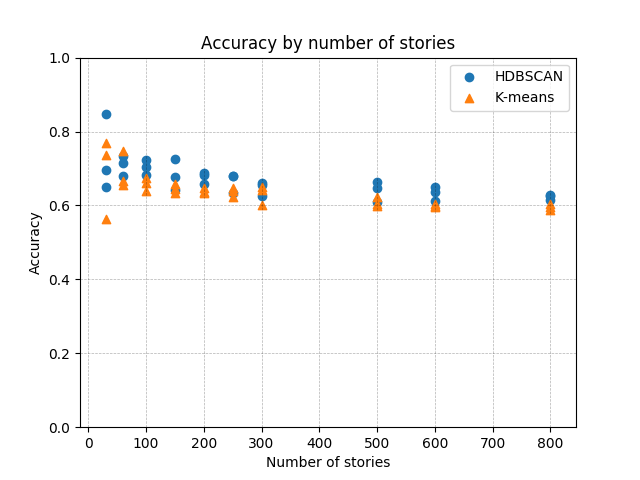
\includegraphics[width=0.5\textwidth]{accuracy_kmeans_hdbscan}
    \caption{Comparison of the average accuracy between K-means and HDBSCAN}
    \label{fig:accuracy_kmeans_hdbscan}
\end{figure}

While HDBSCAN and K-means provide a similar accuracy, the biggest difference can be noted in the processing time in relation to an increasing number of samples. K-means has a time complexity of $O(n^2)$ in contrast to HDBSCAN with a time complexity of $O(nlog(n))$, which is demonstrated by figure \ref{fig:processing_time_kmeans_hdbscan}. Although running the evaluation has also shown the space complexity for HDBSCAN to be substantially higher for larger amounts of samples than with K-means. Trying to run HDBSCAN with 100'000 news articles caused in a memory error, even with 64GB of RAM, while K-means was able to complete the clustering.

% TODO measure memory?

\begin{figure}[h]
    \centering
    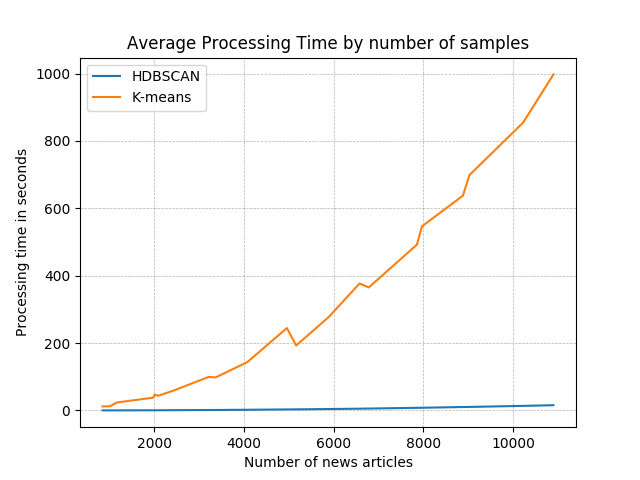
\includegraphics[width=0.5\textwidth]{processing_time_kmeans_hdbscan}
    \caption{Processing time in seconds }
    \label{fig:processing_time_kmeans_hdbscan}
\end{figure}

Figure \ref{fig:cluster_difference_samples} shows, that the difference between predicted over the true number of clusters is fairly low and appears to be roughly linear with the overall number of clusters.  

\begin{figure}[h]
    \centering
    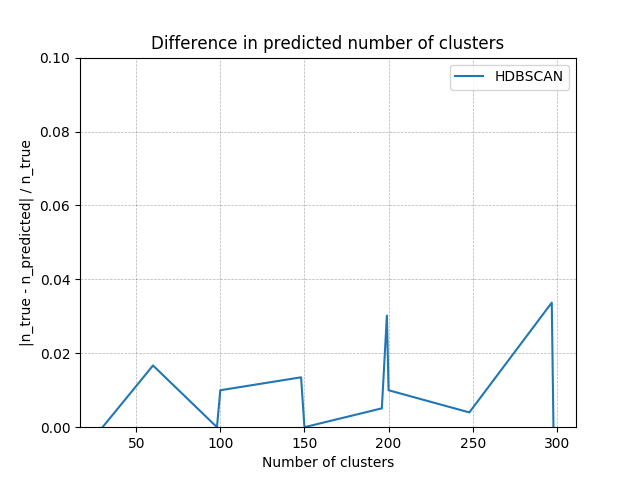
\includegraphics[width=0.5\textwidth]{cluster_difference_samples}
    \caption{Ratio of difference over predicted with true number of clusters}
    \label{fig:cluster_difference_samples}
\end{figure}

So far we have looked at data provided by the most accurate parameter combination. Figure \ref{fig:hdbscan_parameters} shows the accuracies of two essential parameters when working with HDBSCAN. The metric is used when calculating the distances between instances in a feature array. For this evaluation we only consider the metrics $cosine$ and $euclidean$, since other available metrics are either unable to work with sparse matrices or the score was too low, while taking significantly longer to calculate. The comparison in figure \ref{fig:hdbscan_parameters} clearly shows the difference in accuracy between both metrics. Additionally we found that the vectorizer used for the feature matrix, has an big impact on the $euclidean$ metric, while the scores using $cosine$ were relatively stable. Using the $CountVectorizer$ caused the accuracy to drop significantly in combination with the $euclidean$ metric, while using $TFIDF$ gives the accuracies as shown in Figure \ref{fig:hdbscan_parameters}. The second parameter defines the minimum size of a cluster and depends heavily on the dataset. In our case we have clusters with sizes ranging from 1 to 450. We consider clusters with size one as noise, which is why we start with two and evaluate sizes up to nine. The evaluation shows, that a score too low such as $min\_cluster\_size=2$, will lead to an low accuracy, since the granularity of clustering starts to get too small. Increasing the $min\_cluster\_size$ eventually leads to another drop in accuracy, since we start to loose more clusters the higher the minimum size is set to. The optimum results are achieved with a $min\_cluster\_size$ of 4 or 5.

\begin{figure}[h]
    \centering
    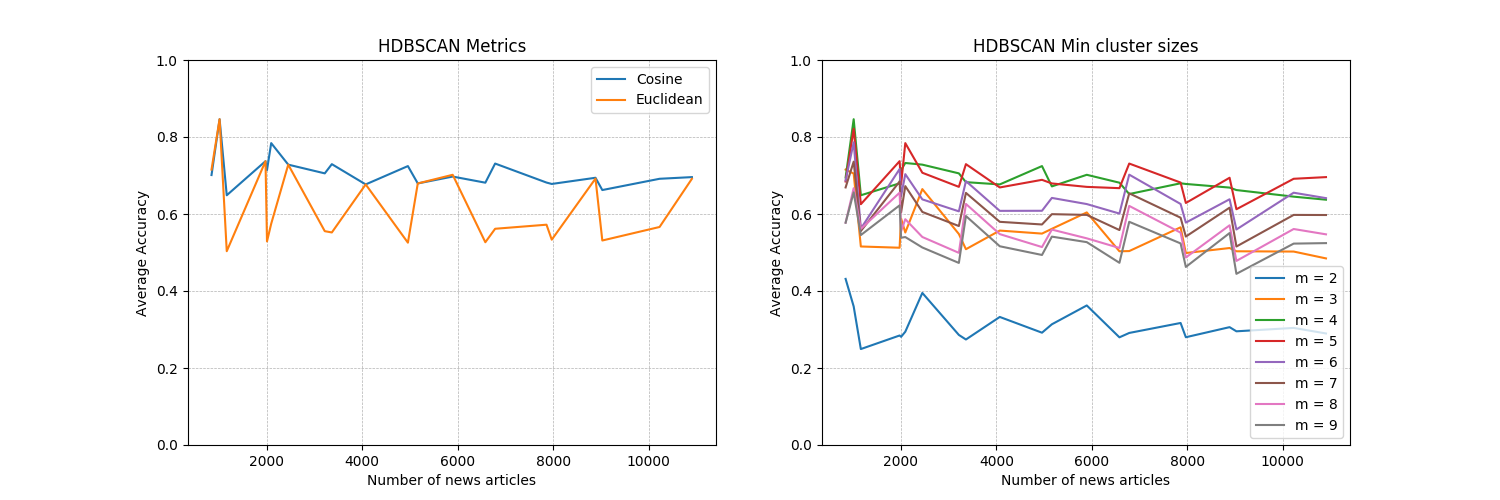
\includegraphics[width=1\textwidth]{hdbscan_parameters}
    \caption{Accuracies for different parameters}
    \label{fig:hdbscan_parameters}
\end{figure}


Being able to handle noise is one of the advantages of HDBSCAN has over the other clustering algorithms. It is reasonable to expect to have a lot of noise in the incoming stream of news articles, once the algorithm is applied in an online setting. However this evaluation is done with a labeled static dataset, containing a minimum amount of noise. The noise ratio shown in Figure \ref{fig:noise_ratio_samples} is higher, than we would expect from the test data. One reason is that clusters lower than the threshold $min\_cluster\_size$ will be classified as noise. Although considering the optimum accuracy can be obtained by using $min\_cluster\_size=5$ only approximately $2\%$ of clusters will drop out due to the minimum size. This does explain the noise ratio of $25\%$. Another possibility is that the data does contain a high number of noisy news articles, but considering the initial substantial effort into cleaning the test data, we estimate the noise ratio to be in the single digit range, rather than anywhere near $20\%$ to $30\%$. 

% experiment with min_samples

\begin{figure}[h]
    \centering
    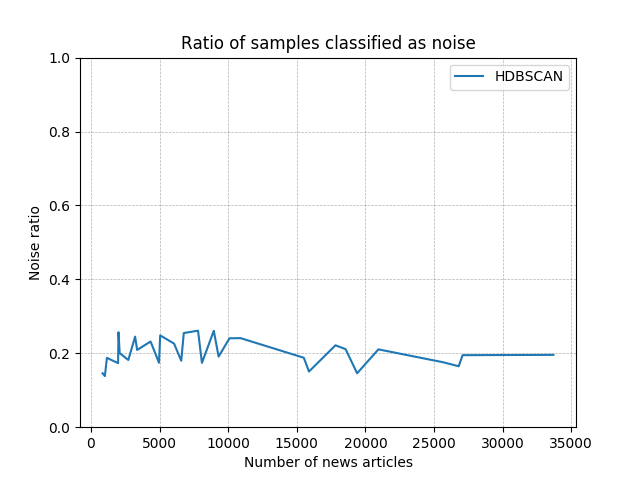
\includegraphics[width=0.5\textwidth]{noise_ratio_samples}
    \caption{Number of news articles classified as noise.}
    \label{fig:noise_ratio_samples}
\end{figure}


The evaluation has shown HDBSCAN to be a good candidate to use for news clustering. It provides an better accuracy than K-means, while being much faster to process. The predicted number of clusters is consistent with an increasing number of samples and fairly close the truth. The ideal parameters for our dataset are $cosine$ as the distance metric and 4 or 5 as the minimum cluster size. On the flip side the noise ratio is quite high and the space complexity is problematic with larger datasets. Overall HDBSCAN provides a acceptable accuracy, while still leaving room for major improvements.

\subsection{Evaluation of online clustering}

TODO new topic, topic extended

\begin{figure}[h]
    \centering
    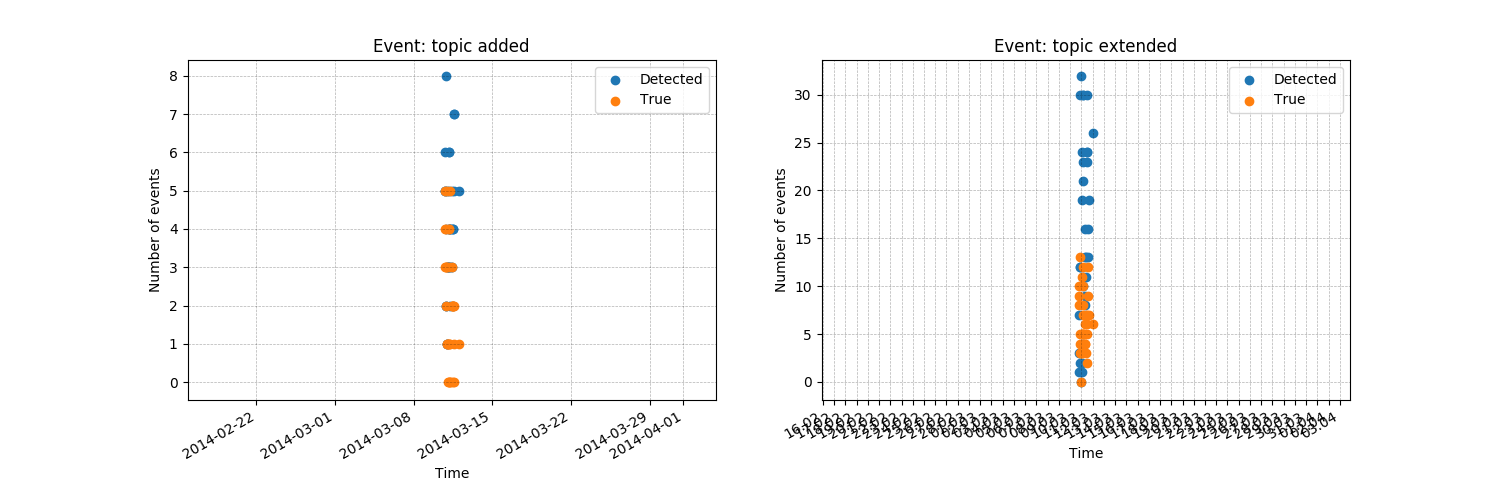
\includegraphics[width=1\textwidth]{event_detection_by_date}
    \caption{Comparison between detected and true events}
    \label{fig:event_detection_by_date}
\end{figure}

\begin{figure}[h]
    \centering
    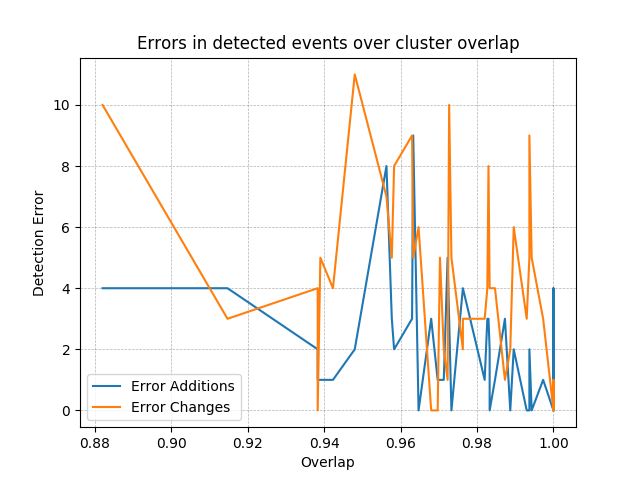
\includegraphics[width=0.5\textwidth]{event_detection_overlap}
    \caption{Plot work in progress}
    \label{fig:event_detection_overlap}
\end{figure}

% analyse overlap size
% show incoming news articles
% show deletion events on full clusterings